\documentclass[12pt,addpoints]{exam}
\usepackage{amsmath}
    \DeclareMathOperator\cis{cis}
\usepackage{amssymb}
\usepackage{tikz}
\usepackage{pgfplots}
    \pgfplotsset{compat=newest}
    
\tikzset{answer/.style={draw,text opacity=0,opacity=0}}
\let\oldprintanswers\printanswers
\def\printanswers{\oldprintanswers\tikzset{answer/.style={text opacity=1,opacity=1,color=red}}}

\usepackage{parskip}

\usepackage{caption}
\DeclareCaptionFormat{empty}{#1}
\renewcommand*\figurename{\sffamily\bfseries Figure}

\setlength{\parindent}{0em}
\setlength{\parskip}{1em}

\usepackage{lastpage}
\footer{}{\iflastpage{\sffamily page~\textbf{\thepage}~of~\textbf{\pageref{LastPage}~--~\textbf{\textit{end of booklet}}}}{\sffamily page~\textbf{\thepage}~of~\textbf{\pageref{LastPage}}}}{\iflastpage{}{\oddeven{\sffamily PLEASE TURN OVER}{}}}

\usepackage{xcolor}
\colorgrids
\definecolor{GridColor}{gray}{0.7}

\makeatletter
\def\fillwithgrid#1{
    \vspace{1ex}
    \fullwidth{
  \begingroup
  \ifhmode
    \par
  \fi
  \hrule height \z@
  \nobreak
  \setlength{\@tempdima}{\gridsize}
  \addtolength{\@tempdima}{\gridlinewidth}
  \setlength{\@tempdimb}{\gridsize}
  \addtolength{\@tempdimb}{-\gridlinewidth}
  \setbox0=\hbox{%
    \rlap{\vrule height \gridsize depth \gridlinewidth width \gridlinewidth}%
    \rlap{\vrule height \gridsize depth -\@tempdimb width \@tempdima}%
    \vrule height 0pt depth \gridlinewidth width \@tempdima
    \llap{\vrule height \gridsize depth \gridlinewidth width \gridlinewidth}%
  }%
  \wd0=\gridsize
  \dp0=0pt
  \setbox1=\hbox to \textwidth{%
    \color@begingroup
    \if@colorgrids
      \color{GridColor}%
    \fi
    \hskip \@totalleftmargin \leaders\copy0\hfil \kern\gridlinewidth
    \color@endgroup
  }
  \cleaders \copy1 \vskip #1 \kern \gridlinewidth \hbox{}%
  \endgroup
  }
      \vspace{-1ex}\droppoints
}

\renewenvironment{solutionorgrid}[1][0pt]%
  {%
    \@insolutiontrue % cancelled by the end of the environment
    \@addpointsfalse % cancelled by the end of the environment
    \ifprintanswers
      \begingroup
      \Solution@Emphasis
      \begin{TheSolution}%
    \else
      \ifcancelspace
        % Do nothing
      \else
        \par
        \penalty 0
        \fillwithgrid{#1}%
      \fi
      \setbox\z@\vbox\bgroup
    \fi
  }{%
    \ifprintanswers
      \end{TheSolution}%
      \endgroup
                \droppoints
    \else
      \egroup
    \fi
  }%
\makeatother


\renewcommand{\d}{\mathrm{d}}

\usepackage{geometry}
    \geometry{
        a4paper,
        margin=2.5cm,
        right=2cm,
        bottom=3cm,
        headheight=14.5pt,
        marginparsep=0mm
    }

\marksnotpoints
\qformat{\textbf{Question~\thequestion}\qquad\qquad(\totalpoints{}~\points)\hfill\vrule depth 3ex width 0pt}
\setlength{\rightpointsmargin}{3cm}
\pointsdroppedatright
\pointformat{(\thepoints)}

\renewcommand{\questionshook}{
    \leftmargin=0pt
    \labelwidth=-\labelsep
}

\usepackage{enumitem}

\renewcommand{\subpartlabel}{(\thesubpart)}

\renewcommand{\solutiontitle}{\noindent\textbf{Solution:}~}
\SolutionEmphasis{\color{red}\sffamily\small}

\usepackage{tkz-euclide}

\newcommand{\blankpage}{
    \pagebreak
    \null
    \vfill
    \begin{center}
        BLANK PAGE
    \end{center}
    \vfill
    \pagebreak
}

\newcommand{\linedpage}{
    \pagebreak
    \begin{framed}
        \lines{26}
    \end{framed}
}

\usepackage{siunitx}

% Replace include/crest.png with your school crest
\newcommand{\school}{% Type in the name of your school
School of Rock
}
\newcommand{\course}{% Type in the course name
Specialist Mathematics
}
\newcommand{\taskyear}{% Replace "\the\year{}" with the year, else it will put in the current year
\the\year{}
}
\newcommand{\taskname}{% Type in the task name/number
Task 1
}
\newcommand{\totaltime}{% Type in the total time in minutes
120 minutes
}

%\printanswers

\begin{document}
\sffamily
\begin{coverpages}
{
\renewcommand\labelitemi{$\vcenter{\hbox{\tiny$\bullet$}}$}
\setlist[itemize]{
    itemsep=-1em,
    align=parleft,
    leftmargin=1em,
    labelwidth=0.5em,
    topsep=0em
}
    \begin{minipage}{0.25\linewidth}
        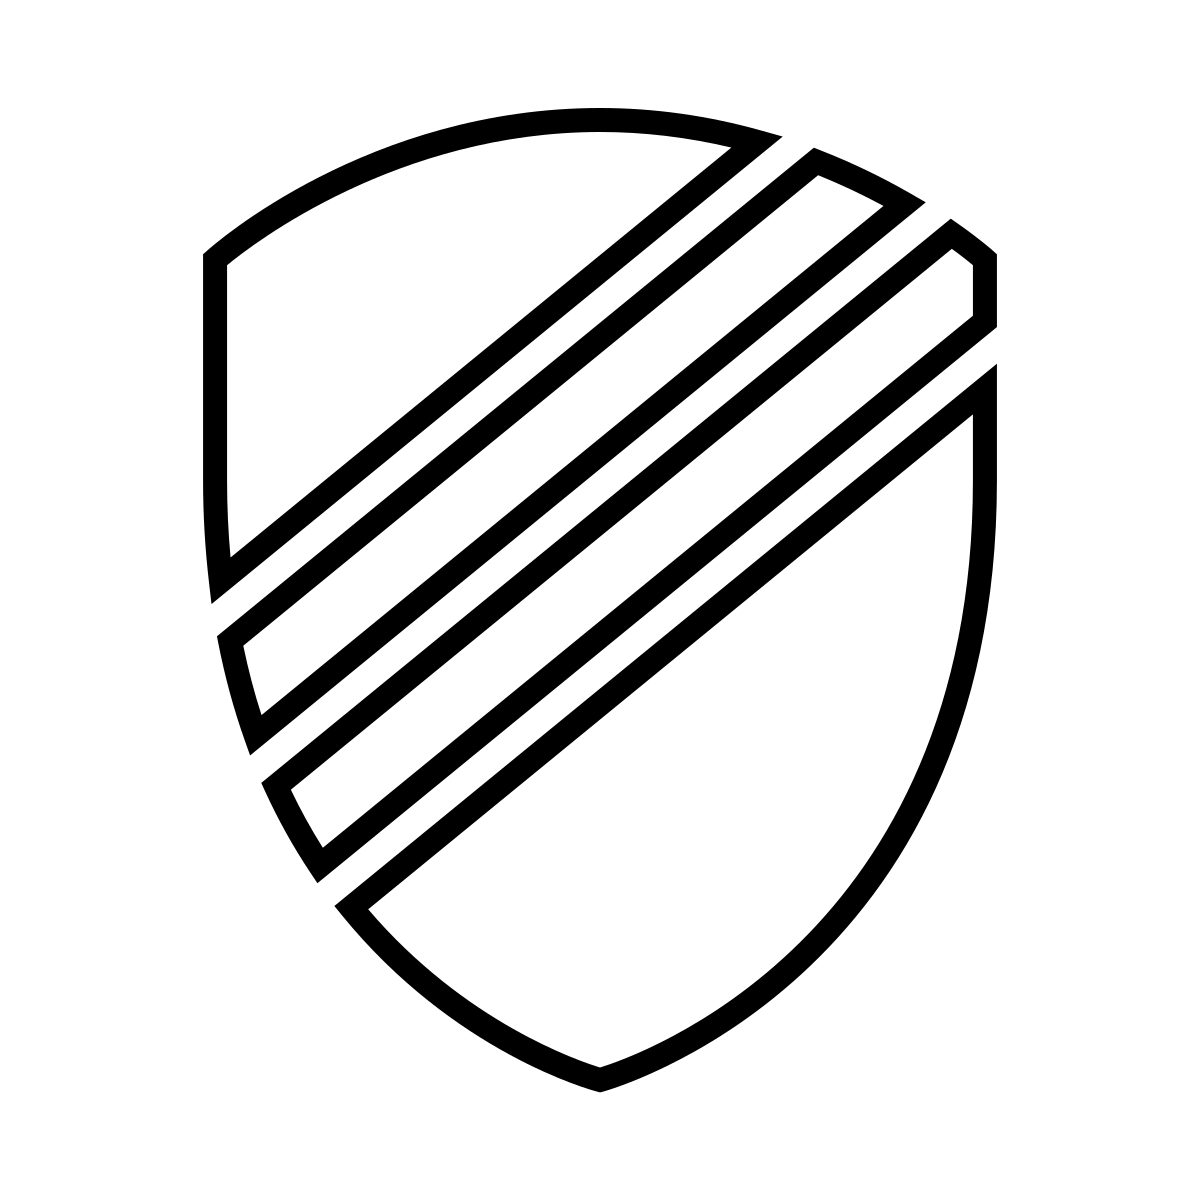
\includegraphics[width=2.9cm]{include/crest.png}
    \end{minipage}
    \begin{minipage}{0.7\linewidth}
        \begin{flushright}
        {\large
            \school\\\vspace{1ex}
            Mathematics Department\\\vspace{1ex}
            \course\\\vspace{1ex}
            \taskyear\\\vspace{1ex}
            \taskname\\\vspace{1ex}
        }
            \end{flushright}
    \end{minipage}
    
    \vspace{1cm}
    \textbf{Question booklet}
    \begin{itemize}
        \item Answer \textbf{\textit{all}} questions
        \item Write your answers in this question booklet
        \item Allow approximately \totaltime minutes
        \item Approved calculators may be used
    \end{itemize}
    \vfill
    \textbf{Examination information}\par
    \textbf{Materials}
    \begin{itemize}
        \item Question booklet
        \item Formula sheet
    \end{itemize}
    \textbf{Instructions}
    \begin{itemize}
        \item Show appropriate working and steps of logic in the question booklets
        \item State all answers correct to three significant figures, unless otherwise instructed
        \item Use black or blue pen
        \item You may use a sharp dark pencil for diagrams
    \end{itemize}
    \textbf{Total time:} \totaltime\\
    \textbf{Total marks:} \numpoints
    \vfill
    Student Name:\ \parbox[b][2em][b]{6cm}{\dotfill}
    \hfill
    Class:\ \parbox[b][2em][b]{5cm}{\dotfill}
}
\end{coverpages}
\addtocounter{page}{1}

%\blankpage
\begin{questions}
\question
\begin{parts}
    \part[1]
    Write $-1+i\sqrt{3}$ in $r\cis\theta$ form.
    \begin{solutionorgrid}[2cm]
        $2\cis\left(\dfrac{2\pi}{3}\right)$
    \end{solutionorgrid}
%    \fillwithgrid{2cm}
    \part
    Consider the complex number $z_1=x+iy$, where $x>0$, $y>0$, and $x>y$.\par
    The complex number $z_1$, which lies in the first quadrand of the Argand diagram, is shown in Figure 1.
    \begin{figure}[h]
        \centering
        \begin{tikzpicture}
            \draw[stealth-stealth] (-4,0) -- (4,0) node[right] {$\text{Re}(z)$};
            \draw[stealth-stealth] (0,-1) -- (0,4) node[above] {$\text{Im}(z)$};
			\tkzDefPoint(0,0){O}
			\tkzDefPoint(1.8,1){z1}
			\tkzDefPoint(1.8,0){z1x}
			\tkzDefPoint(0,1){y}
			\tkzDefPoint(-3.6,2){z2}
			\tkzDefPoint(-3.6,0){z2x}
			\tkzDefPoint(0,2){z2y}
			\tkzDrawSegment[-stealth](O,z1)
			\tkzLabelPoint[right](z1){$z_1$}
			\tkzDrawSegment[dashed](z1x,z1)
			\tkzLabelSegment[right](z1x,z1){$y$}
			\tkzLabelSegment[below](O,z1x){$x$}
			\tkzLabelPoint[below left](O){$0$}
			\draw[answer,opacity=0] (O) -- (z2);
			\tkzDrawSegment[-stealth,answer](O,z2)
			\tkzLabelPoint[left,answer](z2){$z_2$}
			\tkzLabelAngle[answer,pos=1.25](y,O,z2){$\frac{2\pi}{3}$}
			\tkzMarkAngle[mark=none,-stealth,answer,size=.75](z1,O,z2)
			\tkzDrawSegment[dashed,answer](z2x,z2)
			\tkzLabelSegment[left,answer](z2x,z2){$2y$}
			\tkzDrawSegment[dashed,answer](z2y,z2)
			\tkzLabelSegment[above,answer](z2y,z2){$2x$}
        \end{tikzpicture}
        \caption[]{}
    \end{figure}
    \begin{subparts}
        \subpart[1]
        Let $z_2=(-1+i\sqrt{3})z_1$.\par
        Using part (a), show that $|z_2|=2|z_1|.$
        \begin{solutionorgrid}[4cm]
            \[\begin{aligned}
                |z_2|&=|-2+i\sqrt{3}||z_1|\\
                &=|2\cis\left(\frac{2\pi}{3}\right)||z_1|\\
                &=2|z_1|
            \end{aligned}\]
        \end{solutionorgrid}
        \subpart[2]
        On the Argand diagram in Figure 1, draw $z_2$.\par
        \droppoints
    \end{subparts}\newpage
    \part[2]
    Use the triangle inequality to show that $|z_1-z_2|<3|z_1|$.
    \fillwithgrid{4cm}
\end{parts}
\newpage
\question
Figure 2 shows a diagram of an elliptical-shaped oil spill that is expanding in area on the ocean surface.\par
The area of an ellipse is $A=\pi ab$, where $a$ and $b$ are measurements on the axes of symmetry, as shown in Figure 2.

    \begin{figure}[h]
        \centering
        \begin{tikzpicture}
            \draw (0,0) ellipse (30 mm and 15 mm);
            \draw[stealth-stealth] (0,0) -- (3,0) node[midway,below]{$a$};
            \draw[stealth-stealth] (0,0) -- (0,1.5) node[midway,left]{$b$};
        \end{tikzpicture}
        \caption[]{}
    \end{figure}
    
The rate of change of the area of the lliptical oil spill is given by $\dfrac{\d A}{\d t}$. It may be assumed that the elliptical shape is maintained as the oil spill expands.
\begin{parts}
    \part[2]
    Show that $a\dfrac{\d b}{\d t}=\dfrac{1}{\pi}\dfrac{\d A}{\d t}-b\dfrac{\d a}{\d t}$.
    \fillwithgrid{3cm}
    \part
    Consider the instant when the area $A$ is $12$ \unit{m^2}.
    \begin{subparts}
        \subpart[1]
        Show that $a=\dfrac{12}{\pi b}$
        \fillwithgrid{1.5cm}
        \newpage
        \subpart[3]
        The area of the oil spill is expanding at a rate of $2$ \unit{m^2.s^{-1}} at the instant when $$A=12~\unit{m^2},\ b=2~\unit{m},\ \text{and}\ \frac{\d a}{\d t}=0.5~\unit{m.s^{-1}}.$$
        Find the \textbf{\textit{exact}} value of $\dfrac{\d b}{\d t}$ at this instant.
        \fillwithgrid{5.5cm}
    \end{subparts}
\end{parts}
\end{questions}
\end{document}